%!TEX root = ../00_main.tex

%
\begin{figure*}[ht]
    \captionsetup[subfigure]{labelformat=empty} % stop subcaption writing "(a)""
    \captionsetup{subrefformat=parens} % add parentheses to \subref
    \centering
    \begin{subfigure}[t]{\columnwidth}
        \inlinelabel{a}{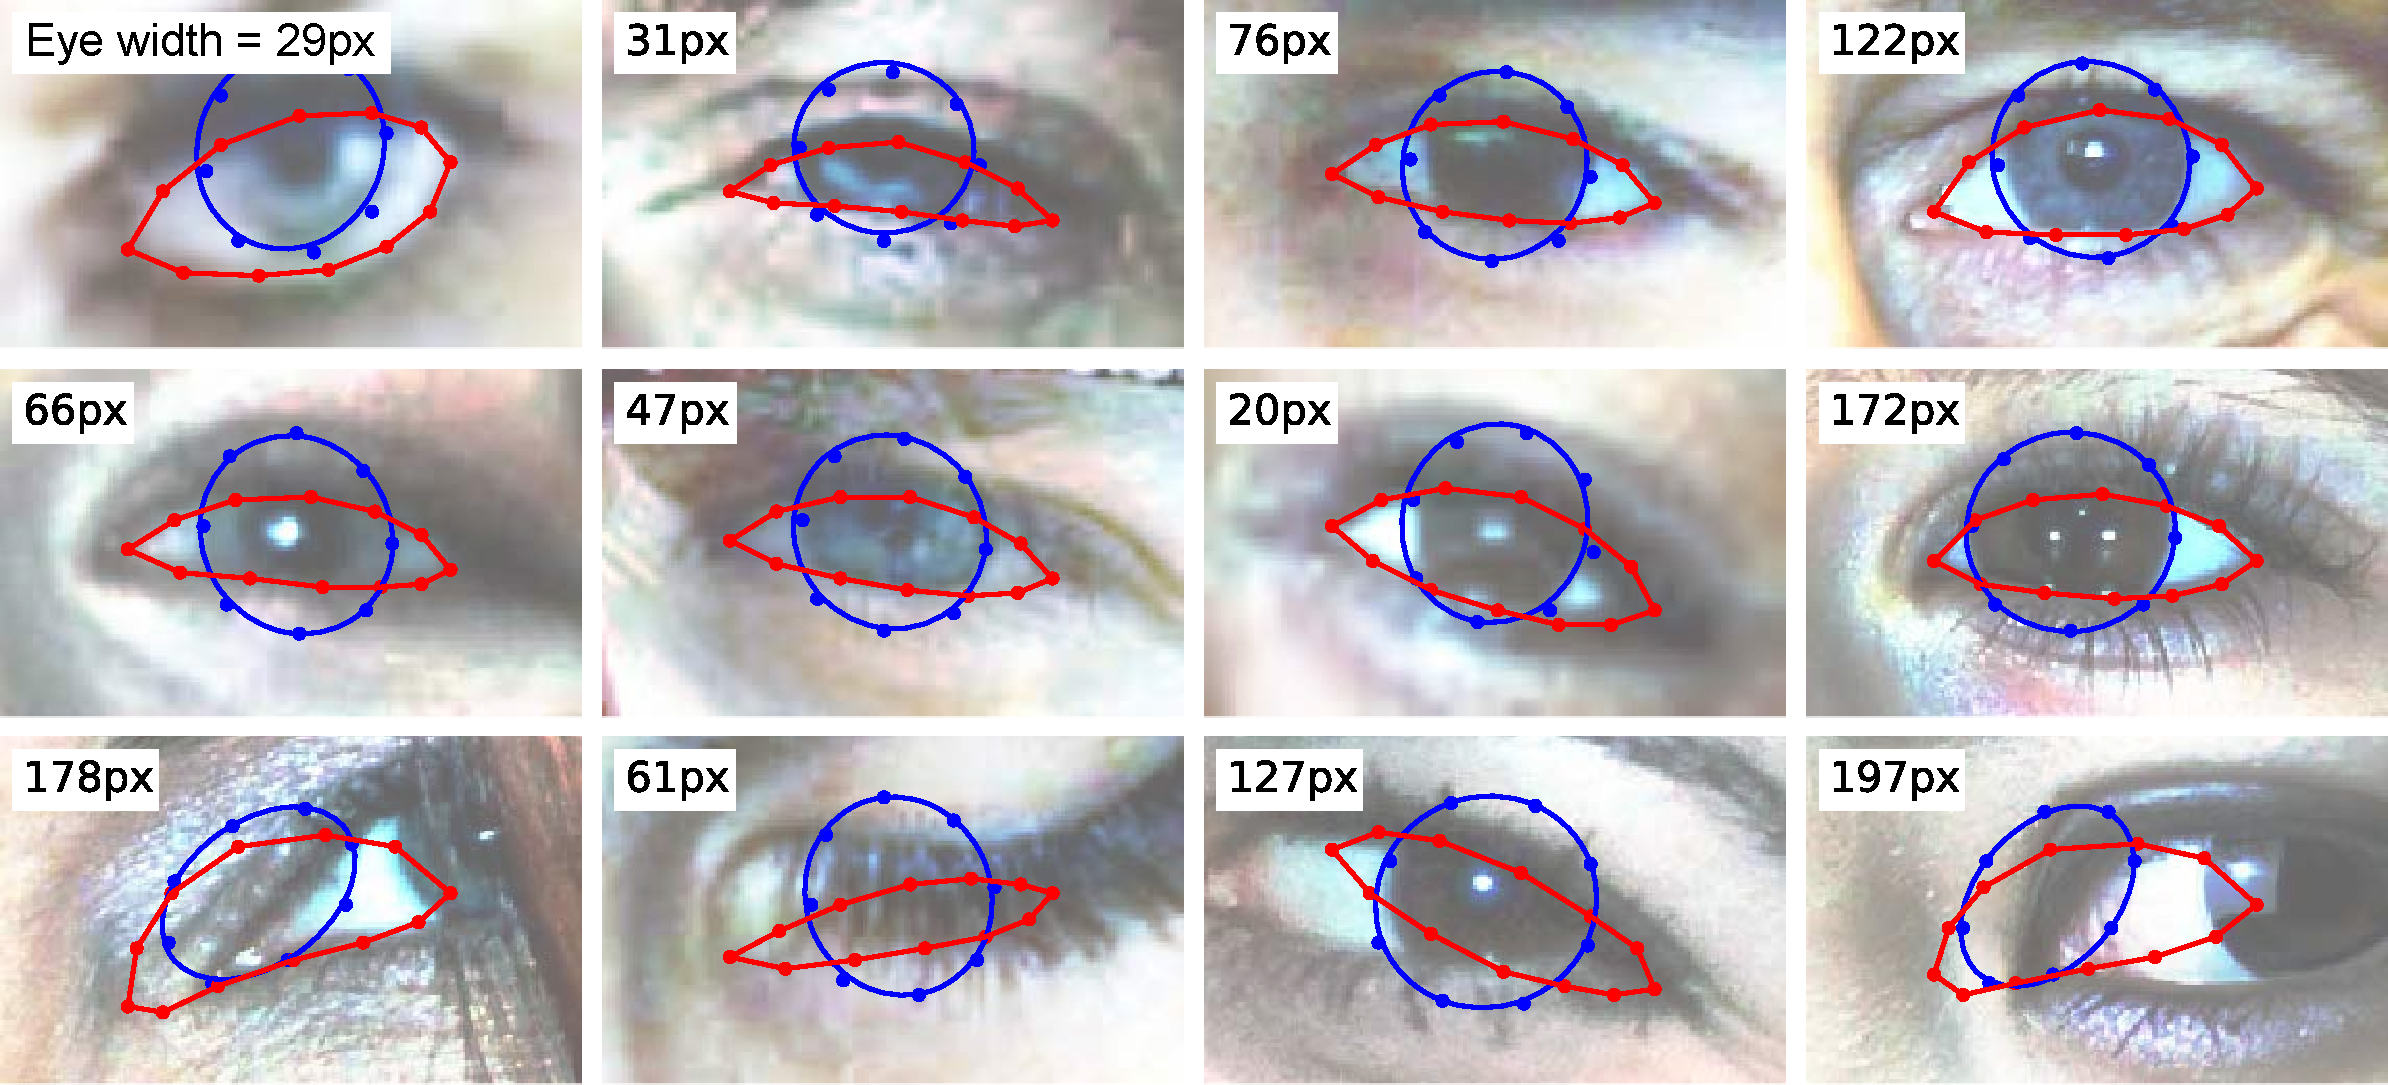
\includegraphics[width=\textwidth]{fits_300W}}
        \caption{}\label{fig:fits_300W}
    \end{subfigure}
    \hfill
    \begin{subfigure}[t]{\columnwidth}
        \inlinelabel{b}{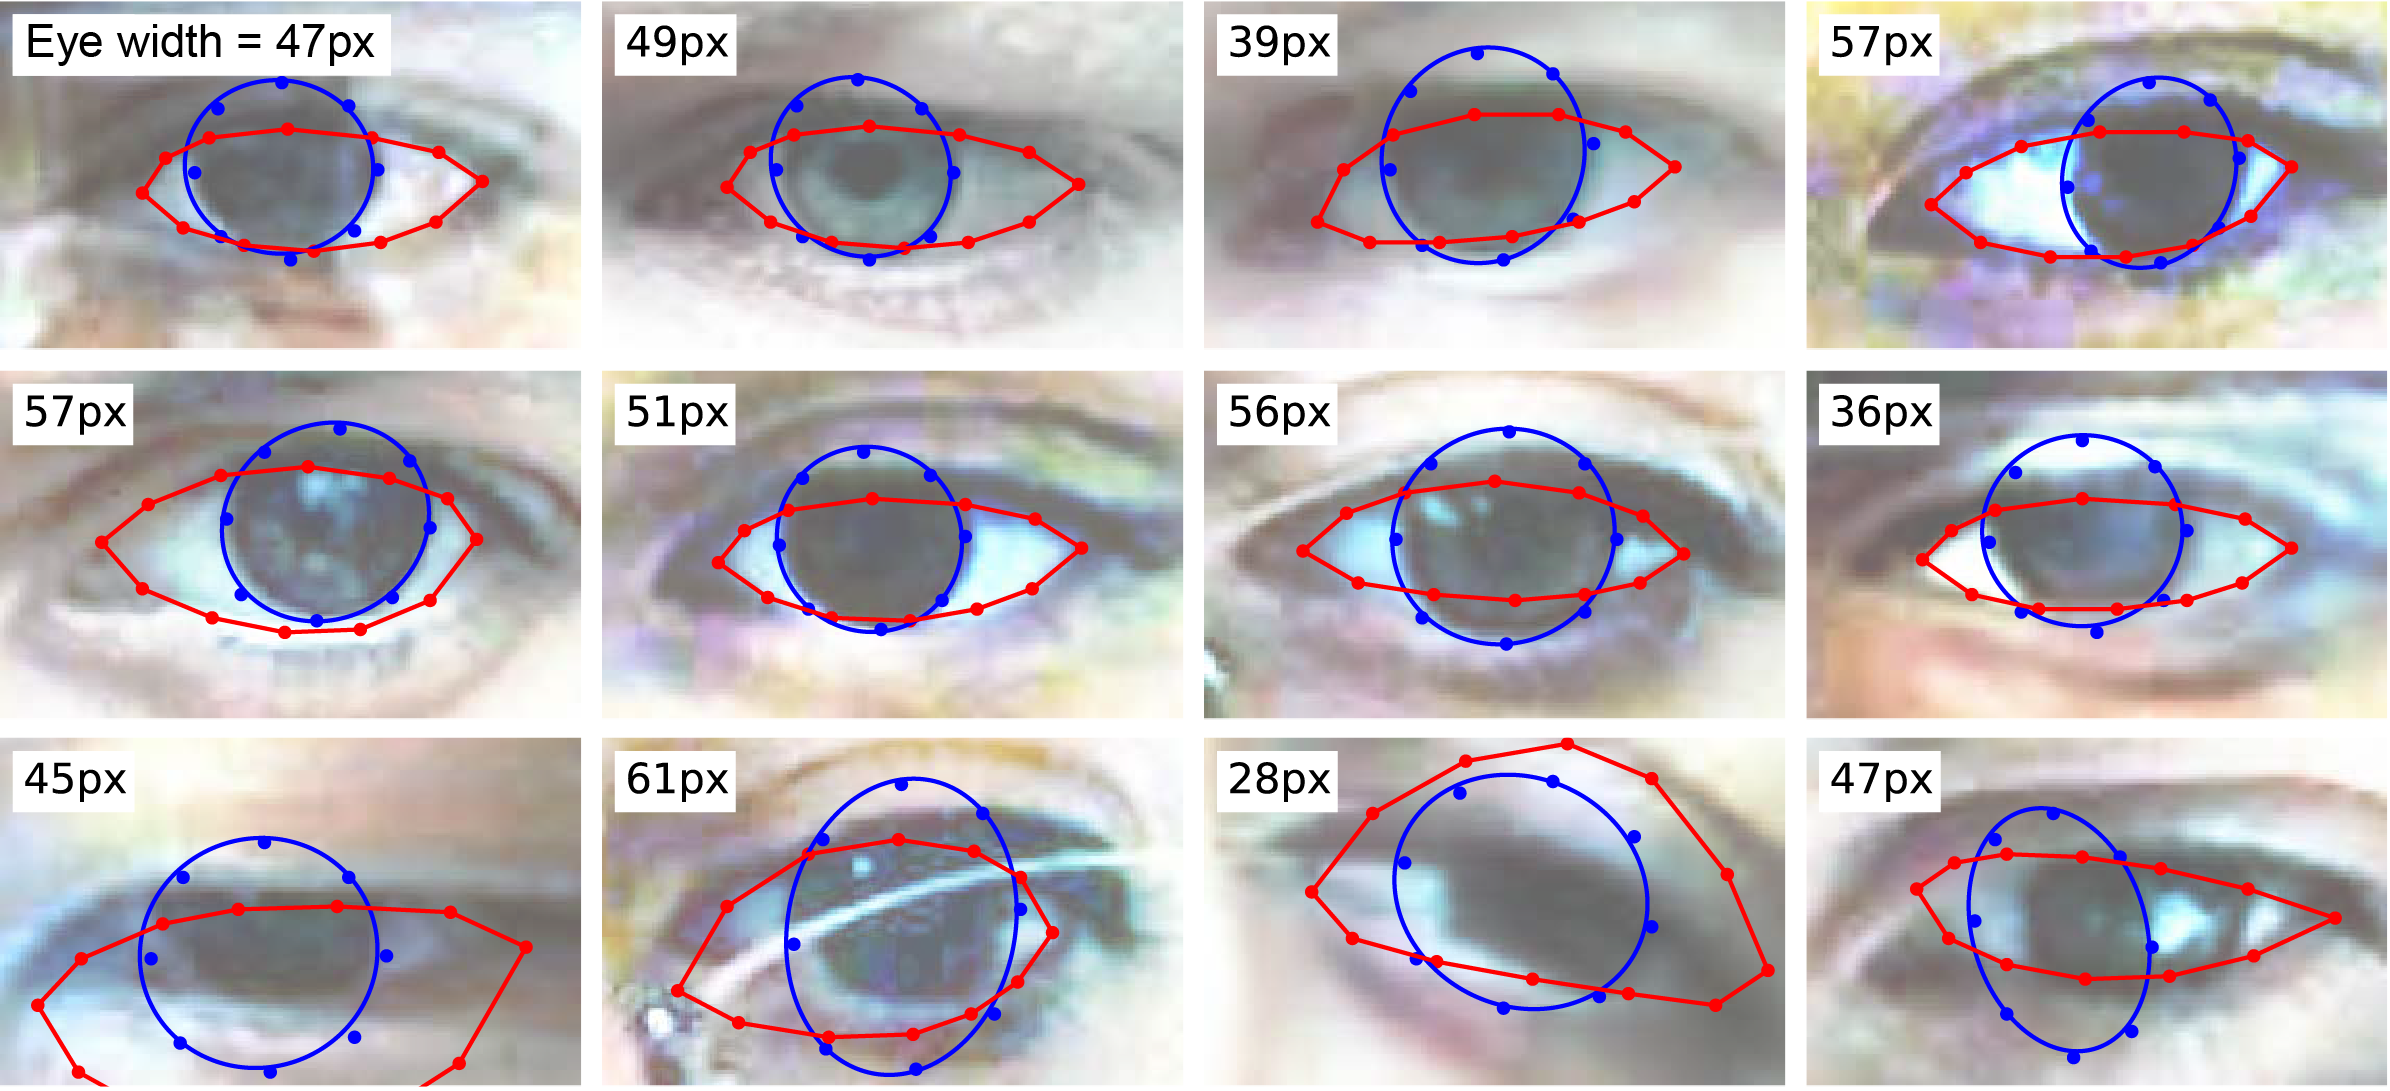
\includegraphics[width=\textwidth]{fits_MPII}}
        \caption{}\label{fig:fits_MPII}
    \end{subfigure}
    \par\vspace{-28pt}
    \caption{Example fits of our eye-CLNF trained on \dataset on in-the-wild images \subref{fig:fits_300W} and webcam images \subref{fig:fits_MPII}. The top two rows illustrate successful eye-shape registration, while the bottom rows illustrate failure cases, including unmodelled occulsions (hair), unmodelled poses (fully closed eye), glasses, and incorrect model initializaion.}
    \label{fig:example_fits}
\end{figure*}